% Provenance (never printed): old premiere S material on the history of plate
% tectonics (from continental drift to seafloor spreading: the ridges, the
% magnetic stripes, the ages of the drilled floor); see
% sources/book2/PROVENANCE.md. Profiles are computed in
% figdata/grade-11/magnetic_stripes.py, the age map in seafloor_age.py, the
% drilling fit in sediment_ages.py.
\chapter{Dari Pergeseran Benua sampai Pemekaran Dasar Samudra}\label{ch:g11:drift-to-spreading}

Pada awal tahun 1950-an, di laboratorium Lamont milik Universitas Columbia,
seorang ahli geologi muda bernama Marie Tharp duduk di depan deretan angka yang
panjang. Setiap angka adalah kedalaman Atlantik Utara, yang diukur dengan perum
gema sebuah kapal, satu demi satu di sepanjang lintasan kapal itu. Dengan
memplot angka-angka itu satu per satu, ia menggambar bentuk dasar samudra di
sepanjang lintasan kapal-kapal yang telah menyeberangi samudra itu. Di tengah
samudra, dasarnya naik menjadi barisan pegunungan --- dan pada setiap lintasan,
di sepanjang puncak barisan itu, dasarnya turun lagi ke dalam sebuah celah yang
dalam, seolah-olah pegunungan itu telah terbelah di tengahnya. Bab ini
mengikuti bagaimana pengukuran-pengukuran dasar samudra seperti itu mengubah
sebuah gagasan yang ditolak, yaitu pergeseran benua, menjadi sebuah teori:
dasar samudra dibuat di punggung-punggung samudra dan bergerak menjauhinya,
dan dasar itu membawa dalam batuannya catatan umurnya sendiri.
% ledger: aip:tharp, aip:featureless, usgs:echo-sounding

\begin{recall}
Pergeseran benua adalah gagasan bahwa benua-benua bergerak; Alfred Wegener
mempertahankannya sejak 1912 dengan kecocokan garis pantai, fosil, batuan, dan
iklim purba, tetapi tidak dapat menjelaskan apa yang menggerakkannya. Permukaan
Bumi tersusun atas lempeng-lempeng kaku, yang bertemu di batas divergen,
konvergen, dan transform; lempeng-lempeng itu bergerak beberapa sentimeter
setahun, dan $\qty{1}{cm}$ setahun sama dengan $\qty{10}{km}$ per sejuta tahun
(Buku 1, kelas 7). Dasar samudra memiliki paparan benua, dataran abisal,
punggung samudra, dan palung samudra (Buku 1, kelas 8). Bumi memiliki medan
magnet, dengan kutub utara dan kutub selatan magnetik, yang diikuti jarum
kompas; pulsa bunyi yang dikirim ke dalam air kembali sebagai gema setelah
selang waktu yang memberikan jaraknya (buku-buku fisika).
\end{recall}

\section{Mengapa pergeseran benua ditolak}

Bukti-bukti Wegener memperlihatkan bahwa benua-benua dahulu pernah bersatu.
Yang tidak diperlihatkannya adalah bagaimana benua-benua itu dapat bergerak.
Wegener membayangkan benua-benua membajak batuan dasar samudra, dan para ahli
fisika menjawab bahwa tidak ada gaya yang dikenal yang dapat mendorong sebuah
benua menembus batuan padat tanpa menghancurkannya. Selama setengah abad,
sebagian besar ahli geologi menyimpulkan bahwa benua-benua sama sekali tidak
bergerak.
% ledger: usgs:wegener-1912, usgs:jeffreys (Book 1 rows)

Ada dua hal yang belum ada. Yang pertama adalah mekanismenya. Yang kedua, yang
kemudian mengarah ke yang pertama, adalah pengetahuan tentang dasar samudra,
yang meliputi sebagian besar permukaan Bumi dan yang, pada tahun 1912, hampir
belum pernah dilihat siapa pun: dasar samudra dianggap berupa dataran yang
hampir tanpa bentuk.
% ledger: aip:tharp, aip:featureless

\section{Memetakan dasar samudra}

Perum gema mengirim pulsa bunyi yang singkat dari lambung kapal ke dasar laut
dan mengukur waktu gemanya. Bunyi merambat melalui air laut dengan laju
sekitar \qty{1500}{m/s}; pulsa itu turun dan kembali, sehingga selang waktu $t$
berarti kedalaman
\[
  d = \frac{v\,t}{2}.
\]
Selang waktu \qty{6.0}{s}, misalnya, berarti $1500 \times 6.0/2 =
\qty{4500}{m}$ air. Pada abad kesembilan belas, kedalaman diukur satu per satu,
dengan menurunkan tali berpemberat sampai ke dasar. Setelah Perang Dunia
Pertama, perum gema mengambil alih, dan rekaman gemanya memperlihatkan dasar
yang jauh lebih kasar daripada yang dibayangkan siapa pun; pada tahun 1950-an
survei-survei kapal dari banyak negara memperlihatkan bahwa sebuah barisan
pegunungan raksasa di dasar samudra membentang hampir mengelilingi seluruh
Bumi.
% ledger: noaa:sound-seawater, usgs:echo-sounding, usgs:line-soundings

\begin{history}[Marie Tharp dan lembah retakan, 1952]
% ledger: aip:tharp, aip:featureless
Sejak 1947, ahli geofisika Bruce Heezen telah mengumpulkan profil-profil perum
gema melintasi Atlantik Utara. Marie Tharp, yang pada masa itu tidak
diizinkan naik ke kapal-kapal riset, mengubah apa yang belakangan disebutnya
``deretan angka perum yang tak ada habisnya'' menjadi gambar-gambar dasar
laut. Pada tahun 1952, setelah menyusun lintasan-lintasan timur--barat itu
berurutan dari utara ke selatan, ia melihat bahwa satu bentuk berjajar dari
lintasan ke lintasan: sebuah celah di sepanjang puncak Punggung Tengah
Atlantik, yaitu lembah retakan. Heezen mula-mula mengira itu sebuah kesalahan.
Lalu episentrum gempa-gempa bumi di Atlantik, yang diplot pada skala yang
sama, ternyata jatuh di dalam lembah retakan itu sendiri. Peta dasar samudra
dunia buatan Tharp dan Heezen, yang dilukis oleh seniman Heinrich Berann pada
tahun 1977, memberi orang gambaran realistis yang pertama tentang dasar samudra;
pada tahun 1997 Perpustakaan Kongres Amerika Serikat menyebutnya salah satu dari empat
kartografer besar abad kedua puluh.
\end{history}

Punggung-punggung tengah samudra membentuk satu sistem tunggal yang hampir
bersambung, panjangnya sekitar \qty{65000}{km}, dan lebih dari sembilan
persepuluhnya berada di bawah air; puncaknya rata-rata berada \qty{2500}{m} di
bawah permukaan. Di sepanjang Punggung Tengah Atlantik yang lambat, puncaknya
terbelah oleh lembah retakan; di sepanjang Tinggian Pasifik Timur yang lebih
cepat, puncaknya berupa puncak yang mulus dan landai. Gempa-gempa bumi di
samudra mengikuti punggung-punggung itu dengan ketat. Segala sesuatu menunjuk
punggung samudra sebagai tempat sesuatu sedang terjadi --- tetapi apa?
% ledger: noaa:ridge, aip:tharp

\section{Pemekaran dasar samudra}

\begin{history}[Hess dan ban berjalan, 1962]
% ledger: usgs:hess, hess:1962
Pada tahun 1962 Harry Hess, seorang ahli geologi di Universitas Princeton dan
laksamana cadangan angkatan laut, menerbitkan \emph{History of Ocean Basins}.
Ia mengusulkan bahwa batuan panas naik di bawah punggung-punggung samudra dan
menjadi dasar samudra yang baru, yang lalu bergerak menjauh di kedua sisi
seperti ban berjalan, dan tenggelam kembali ke dalam mantel di palung-palung.
Robert Dietz, yang sampai pada gagasan yang sama, memberinya nama: \omterm{def:g11:drift-to-spreading:spreading}{pemekaran
dasar samudra}. Gagasan itu menjelaskan mengapa Bumi tidak membesar meskipun
dasar baru terus dibuat, mengapa begitu sedikit sedimen yang terletak di dasar
samudra, dan mengapa batuan dasar samudra jauh lebih muda daripada batuan
benua.
\end{history}

\begin{definition}[Pemekaran dasar samudra]\label{def:g11:drift-to-spreading:spreading}
Yang disebut \emph{pemekaran dasar samudra}\index{pemekaran dasar samudra}
adalah proses yang membentuk dasar samudra baru di sepanjang puncak punggung
tengah samudra, tempat batuan cair naik dari mantel dan membeku, lalu bergerak
menjauhi punggung itu di kedua sisi, sehingga dasar samudra makin tua dengan
bertambahnya jarak dari punggung itu.
\end{definition}

\begin{definition}[Laju pemekaran]\label{def:g11:drift-to-spreading:spreading-rate}
Yang disebut \emph{laju pemekaran penuh}\index{laju pemekaran} sebuah punggung
samudra adalah laju dua lempeng di kedua sisinya saling menjauh. Yang disebut
\emph{laju setengah pemekaran} adalah laju dasar di satu sisi menjauhi sumbu
punggung. Bila pemekarannya simetris, laju penuh sama dengan dua kali laju
setengahnya.
\end{definition}

Punggung-punggung samudra memekar dengan laju yang sangat berbeda. Punggung
Tengah Atlantik membuka dengan laju \qtyrange{2}{5}{cm} setahun, Tinggian
Pasifik Timur dengan laju \qtyrange{6}{16}{cm} setahun. Dari dasar samudra yang
ada saat ini, sekitar sepertiganya dibuat di punggung yang lambat (laju penuh
\qtyrange{20}{55}{mm} setahun) dan sekitar dua perlimanya di punggung yang
cepat (\qtyrange{75}{180}{mm} setahun).
% ledger: noaa:ridge, seton:rate-classes

Gagasan Hess berani, dan mula-mula hanya sedikit bukti langsung yang
mendukungnya. Bukti itu datang dari dua arah yang tak terduga: kemagnetan dasar
samudra dan sedimen-sedimennya.

\section{Pembalikan magnetik dan dasar laut yang bergaris-garis}

\subsection{Batuan mengingat medan magnet}

Basalt dasar samudra mengandung butir-butir kecil magnetit, yaitu oksida besi
yang bersifat sangat magnetis. Ketika lava basalt meletus, lava itu terlalu
panas untuk mempertahankan magnetisasi yang langgeng; ketika mendingin,
butir-butirnya termagnetisasi sejajar dengan medan Bumi di sekitarnya, dan arah
itu lalu terkunci di dalam batuan.
% ledger: usgs:magnetometers

\begin{definition}[Magnetisasi remanen; suhu Curie]\label{def:g11:drift-to-spreading:remanence}
Yang disebut \emph{suhu Curie}\index{suhu Curie} sebuah mineral magnetis
adalah suhu yang di atasnya mineral itu tidak dapat mempertahankan
magnetisasinya sendiri: sekitar \qty{580}{\celsius} untuk magnetit. Batuan yang
butir-butir magnetisnya mendingin melewati suhu Curie-nya di dalam medan Bumi
mempertahankan magnetisasi yang sejajar dengan medan pada masa itu, yaitu
\emph{magnetisasi remanen}\index{magnetisasi remanen}. Magnetisasi itu bertahan
lama setelah medannya berubah, kecuali batuan itu dipanaskan lagi di atas suhu
Curie.
\end{definition}
% ledger: tarduno:curie

\begin{omfigure}
\begin{tikzpicture}[font=\footnotesize, >={Stealth[length=5pt]}]
  % ground and lava flow
  \fill[lith basalt] (0,0) rectangle (11,0.6);
  \fill[omLithBasalt!45!red!35] (0,0.6) -- (11,0.6) -- (11,1.9) .. controls (9,2.0) and (4,2.15) .. (0,2.05) -- cycle;
  \fill[omLithBasalt!70] (0,1.35) -- (11,1.25) -- (11,1.9) .. controls (9,2.0) and (4,2.15) .. (0,2.05) -- cycle;
  \draw[black!60] (0,1.35) -- (11,1.25);
  \draw[line width=0.8pt] (0,2.05) .. controls (4,2.15) and (9,2.0) .. (11,1.9);
  \draw[black!60] (0,0.6) -- (11,0.6);
  % field lines (northern hemisphere: pointing down to the north)
  \foreach \x in {0.6,2.4,4.2,6.0,7.8,9.6} {
    \draw[->, omDef, line width=0.9pt] (\x,4.0) -- (\x+1.1,2.55);
  }
  \node[anchor=south west, text=omDef] at (0.2,4.05) {medan magnet Bumi};
  % locked grains in the cooled top
  \foreach \x in {0.5,1.3,...,10.5} {
    \draw[->, black, line width=0.6pt] (\x,1.86) -- (\x+0.25,1.53);
  }
  % random grains in the hot interior
  \foreach \x/\a in {0.6/20,1.5/140,2.3/250,3.2/80,4.0/310,4.9/190,5.7/40,6.6/120,7.4/280,8.3/20,9.1/200,10.0/330} {
    \draw[->, black!55, line width=0.5pt] (\x,0.95) -- ++(\a:0.22);
  }
  \node[anchor=west, align=left] at (11.15,1.75) {sudah di bawah \qty{580}{\celsius}:\\butir menyimpan arah medan};
  \node[anchor=west, align=left] at (11.15,0.92) {masih di atas \qty{580}{\celsius}:\\tanpa magnetisasi yang langgeng};
  \node[anchor=west, align=left] at (11.15,0.25) {batuan yang lebih tua};
  \node[anchor=west] at (9.0,4.25) {utara $\rightarrow$};
\end{tikzpicture}

{\small Aliran lava yang sedang mendingin (skematis, belahan bumi utara, tempat
medan magnet mengarah ke utara dan ke bawah). Bagian atas aliran telah
mendingin di bawah \omterm{def:g11:drift-to-spreading:remanence}{suhu Curie} magnetit: butir-butir magnetisnya (panah hitam)
mempertahankan arah medan. Bagian dalamnya, yang masih lebih panas, belum
merekam apa pun; bagian itu akan merekam medan pada saat bagian itu mendingin.}
\end{omfigure}

\subsection{Medan magnet berbalik}

Pada awal abad kedua puluh, Bernard Brunhes (pada tahun 1906) dan kemudian
Motonori Matuyama (pada tahun 1920-an) menemukan bahwa batuan vulkanik terbagi
menjadi dua kelompok. Pada sebagian, magnetisasinya mengarah sama seperti medan
masa kini; pada yang lain magnetisasinya mengarah berlawanan, seolah-olah kutub
utara dan kutub selatan magnetik telah bertukar tempat. Medan itu sendiri
telah berbalik, berulang-ulang.
% ledger: usgs:reversals

\begin{definition}[Pembalikan magnetik; polaritas normal dan terbalik]\label{def:g11:drift-to-spreading:reversal}
Yang disebut \emph{pembalikan magnetik}\index{pembalikan magnetik} adalah
pertukaran kutub utara dan kutub selatan magnetik Bumi. Masa ketika medan
mengarah seperti saat ini adalah masa
\emph{polaritas normal}\index{polaritas normal}; masa ketika medan mengarah
berlawanan adalah masa \emph{polaritas terbalik}\index{polaritas terbalik}.
Batuan yang termagnetisasi selama salah
satu masa itu memiliki polaritas yang sama.
\end{definition}

Lava-lava yang telah ditentukan umurnya memberikan urutan selang-selang
normal dan terbalik: \emph{skala waktu polaritas geomagnetik}. Selang-selangnya
yang panjang dinamai menurut ilmuwan yang mempelajari kemagnetan Bumi
(Brunhes, Matuyama, Gauss, Gilbert); peristiwa-peristiwa pendek di dalamnya,
menurut tempat peristiwa itu pertama kali ditemukan.

\begin{omfigure}
\begin{tikzpicture}
\begin{axis}[width=0.92\linewidth, height=3.2cm, xmin=0, xmax=5.5, ymin=-0.9, ymax=1.9,
  axis y line=none, axis x line*=bottom, xtick={0,0.5,...,5.5}, tick label style={font=\small},
  xlabel={umur (juta tahun)}, label style={font=\small}, clip=false]
\addplot[fill=black, draw=none] table {figdata/out/grade-11-magnetic_stripes-timescale.dat};
\draw[black] (axis cs:0,0) rectangle (axis cs:5.5,1);
\begin{scope}[every node/.style={font=\scriptsize, anchor=south}]
  \node at (axis cs:0.39,1.05) {Brunhes};
  \node at (axis cs:1.68,1.05) {Matuyama};
  \node at (axis cs:3.08,1.05) {Gauss};
  \node at (axis cs:4.74,1.05) {Gilbert};
\end{scope}
\draw[black!60] (axis cs:0.78,1) -- (axis cs:0.78,1.45);
\draw[black!60] (axis cs:2.581,1) -- (axis cs:2.581,1.45);
\draw[black!60] (axis cs:3.58,1) -- (axis cs:3.58,1.45);
\begin{scope}[every node/.style={font=\scriptsize, anchor=north}]
  \node at (axis cs:1.03,-0.05) {Jaramillo};
  \node at (axis cs:1.86,-0.05) {Olduvai};
\end{scope}
\node[font=\scriptsize, anchor=west] at (axis cs:5.55,0.75) {normal};
\node[font=\scriptsize, anchor=west] at (axis cs:5.55,0.25) {(hitam)};
\end{axis}
\end{tikzpicture}

{\small Skala waktu polaritas geomagnetik untuk 5.5 juta tahun terakhir: hitam
untuk \omterm{def:g11:drift-to-spreading:reversal}{polaritas normal}, putih untuk \omterm{def:g11:drift-to-spreading:reversal}{polaritas terbalik}. Selang normal masa
kini bermula \num{780000} tahun yang lalu; ada dua puluh pembalikan dalam lima
juta tahun terakhir. Data: Cande dan Kent (1995).}
\end{omfigure}
% ledger: ck95:chrons

\subsection{Garis-garis di dasar samudra}

Sejak tahun 1950-an, kapal-kapal menarik magnetometer di belakangnya
melintasi samudra, dan mendapati bahwa medan di permukaan laut bukanlah medan
mulus yang diharapkan dari inti Bumi: medan itu sedikit lebih kuat di sini,
sedikit lebih lemah di sana.
% ledger: usgs:magnetometers

\begin{definition}[Anomali magnetik]\label{def:g11:drift-to-spreading:anomaly}
Di suatu titik di permukaan laut, yang disebut
\emph{anomali magnetik}\index{anomali magnetik} adalah kuat medan magnet yang
terukur dikurangi kuat medan yang diharapkan di sana dari medan Bumi saja.
Anomali itu positif di tempat batuan di bawahnya menambah medan, negatif di
tempat batuan itu melawannya. Anomali itu kecil dibandingkan dengan medan itu
sendiri, dan diukur dalam nanotesla (\unit{nT}).
\end{definition}

Bila dipetakan di atas wilayah yang luas, anomali-anomali itu membentuk
garis-garis yang sejajar dengan puncak punggung, berganti-ganti positif dan
negatif, seperti belang zebra --- dan pola di satu sisi punggung adalah
bayangan cermin pola di sisi lainnya.
% ledger: usgs:magnetometers

\begin{history}[Vine dan Matthews, 1963]
% ledger: vm:1963, usgs:magnetometers
Pada September 1963, Fred Vine dan Drummond Matthews menerbitkan sebuah
makalah pendek dalam jurnal \emph{Nature}, berjudul
\emph{Magnetic anomalies over oceanic ridges}. Keduanya menggabungkan
pemekaran Hess dengan pembalikan medan magnet. Jika dasar baru terbentuk di
puncak dan bergerak menjauh selagi medan berbalik, setiap jalur dasar merekam
polaritas pada masa jalur itu mendingin. Dasar samudra menjadi pita
bergaris-garis, yang terbentang di kedua sisi punggung: anomali positif di
atas jalur normal, negatif di atas jalur terbalik, dengan urutan yang sama di
kedua sisi.
\end{history}

\begin{omfigure}
\begin{tikzpicture}
\begin{axis}[hide axis, axis equal image, width=0.94\linewidth, xmin=-320, xmax=420, ymin=-120, ymax=160, clip=false]
  % block faces
  \fill[white] (axis cs:-300,0) -- (axis cs:300,0) -- (axis cs:390,70) -- (axis cs:-210,70) -- cycle;
  \fill[omLithBasalt!25] (axis cs:-300,0) rectangle (axis cs:300,-60);
  \fill[omLithBasalt!45] (axis cs:300,0) -- (axis cs:390,70) -- (axis cs:390,10) -- (axis cs:300,-60) -- cycle;
  \addplot[fill=black!80, draw=none] table {figdata/out/grade-11-magnetic_stripes-block.dat};
  \draw[black] (axis cs:-300,0) -- (axis cs:300,0) -- (axis cs:390,70) -- (axis cs:-210,70) -- cycle;
  \draw[black] (axis cs:-300,0) -- (axis cs:-300,-60) -- (axis cs:300,-60) -- (axis cs:300,0);
  \draw[black] (axis cs:300,-60) -- (axis cs:390,10) -- (axis cs:390,70);
  % ridge axis
  \draw[omRidge, line width=1.6pt] (axis cs:0,0) -- (axis cs:90,70);
  \node[font=\footnotesize, text=omRidge, anchor=south] at (axis cs:90,72) {sumbu punggung};
  % rising magma
  \fill[red!60!orange, opacity=0.75] (axis cs:-12,-60) -- (axis cs:12,-60) -- (axis cs:3,0) -- (axis cs:-3,0) -- cycle;
  \draw[->, >={Stealth[length=5pt]}, red!70!black, line width=1pt] (axis cs:0,-95) -- (axis cs:0,-62);
  \node[font=\footnotesize, anchor=north] at (axis cs:0,-96) {batuan cair naik};
  % spreading arrows
  \draw[->, >={Stealth[length=6pt]}, line width=1.2pt] (axis cs:-90,100) -- (axis cs:-220,100);
  \draw[->, >={Stealth[length=6pt]}, line width=1.2pt] (axis cs:150,100) -- (axis cs:280,100);
  \node[font=\footnotesize, anchor=south] at (axis cs:-155,103) {lebih tua};
  \node[font=\footnotesize, anchor=south] at (axis cs:215,103) {lebih tua};
  % legend
  \fill[black!80] (axis cs:-300,-100) rectangle (axis cs:-280,-88);
  \node[font=\footnotesize, anchor=west] at (axis cs:-276,-94) {polaritas normal};
  \draw[black] (axis cs:-300,-118) rectangle (axis cs:-280,-106);
  \node[font=\footnotesize, anchor=west] at (axis cs:-276,-112) {polaritas terbalik};
\end{axis}
\end{tikzpicture}

{\small Dasar samudra yang bergaris-garis (skematis, dihitung untuk punggung
yang memekar \qty{7.5}{cm} setahun di setiap sisi, selama 4 juta tahun
terakhir). Setiap jalur dasar mempertahankan polaritas medan pada masa jalur
itu mendingin di sumbu; pola di satu sisi adalah bayangan cermin pola di sisi
lainnya.}
\end{omfigure}

\begin{proposition}[Jarak sebuah garis dari sumbu]\label{prop:g11:drift-to-spreading:stripe}
Jika sebuah punggung memekar secara simetris dengan laju setengah $u$ yang
tetap, dasar yang terbentuk di sumbu selama waktu $t$ yang lalu kini terletak
pada jarak
\[
  x = u\,t
\]
di kedua sisi sumbu. Khususnya, batas di antara dua garis yang merekam
pembalikan berumur $t$ terletak pada jarak $u\,t$ di kedua sisi.
\end{proposition}

\begin{proof}
Sepotong dasar yang terbentuk di sumbu selama waktu $t$ yang lalu sejak itu
telah bergerak menjauhi sumbu dengan laju $u$, selama waktu $t$: potongan itu
telah menempuh jarak $u\,t$. Potongan yang terbentuk pada saat yang sama di
sisi lain sumbu bergerak ke arah sebaliknya dengan laju yang sama, dan terletak
pada jarak yang sama. Dasar di kedua sisi sebuah batas pembalikan terbentuk
sesaat sebelum dan sesaat sesudah pembalikan itu, sehingga batas itu terletak
di tempat dasar berumur $t$ terletak: pada $u\,t$.
\end{proof}

Anomali-anomali itu dapat dihitung dari skala waktu. Pada profil-profil di
bawah, lapisan yang termagnetisasi adalah lembaran batuan setebal \qty{1}{km}
yang bagian atasnya terletak \qty{3}{km} di bawah permukaan laut, dibagi
menjadi blok-blok berpolaritas normal dan terbalik menurut proposisi itu; medan
setiap blok di permukaan laut dijumlahkan. Di atas jalur yang lebar, anomalinya
paling kuat di dekat tepi-tepinya, tempat polaritas berubah, dan lebih lemah di
atas bagian tengahnya; tetapi tandanya mengikuti polaritas jalur di bawahnya.

\begin{omfigure}
\begin{tikzpicture}
\begin{axis}[omrecord, name=fast, width=0.92\linewidth, height=5.0cm, xmin=-375, xmax=375, ymin=-820, ymax=560,
  ytick={-400,0,400}, xtick={-300,-200,...,300}, tick label style={font=\small}, label style={font=\small},
  ylabel={anomali (\unit{nT})}, title={\small punggung cepat: laju setengah \qty{7.5}{cm} setahun}, clip=false]
\addplot[fill=black, draw=none] table[y expr=\thisrow{y}*55-700] {figdata/out/grade-11-magnetic_stripes-fastblocks.dat};
\draw[black] (axis cs:-375,-755) rectangle (axis cs:375,-645);
\addplot[omDef, line width=0.9pt] table[x=x_km, y=anomaly_nT] {figdata/out/grade-11-magnetic_stripes-fast.dat};
\draw[black!40] (axis cs:-375,0) -- (axis cs:375,0);
\draw[black!50, densely dashed] (axis cs:268.5,-645) -- (axis cs:268.5,560);
\draw[black!50, densely dashed] (axis cs:-268.5,-645) -- (axis cs:-268.5,560);
\node[font=\scriptsize, anchor=south west, fill=white, inner sep=1pt] at (axis cs:270,-610) {3.58 juta tahun};
\end{axis}
\begin{axis}[omrecord, at={(fast.south)}, anchor=north, yshift=-1.6cm, width=0.92\linewidth, height=5.0cm,
  xmin=-62.5, xmax=62.5, ymin=-820, ymax=560, ytick={-400,0,400}, xtick={-60,-40,...,60},
  tick label style={font=\small}, label style={font=\small},
  ylabel={anomali (\unit{nT})}, xlabel={jarak dari sumbu punggung (\unit{km})},
  title={\small punggung lambat: laju setengah \qty{1.25}{cm} setahun}, clip=false]
\addplot[fill=black, draw=none] table[y expr=\thisrow{y}*55-700] {figdata/out/grade-11-magnetic_stripes-slowblocks.dat};
\draw[black] (axis cs:-62.5,-755) rectangle (axis cs:62.5,-645);
\addplot[omProp, line width=0.9pt] table[x=x_km, y=anomaly_nT] {figdata/out/grade-11-magnetic_stripes-slow.dat};
\draw[black!40] (axis cs:-62.5,0) -- (axis cs:62.5,0);
\draw[black!50, densely dashed] (axis cs:44.75,-645) -- (axis cs:44.75,560);
\draw[black!50, densely dashed] (axis cs:-44.75,-645) -- (axis cs:-44.75,560);
\node[font=\scriptsize, anchor=south west, fill=white, inner sep=1pt] at (axis cs:45,-610) {3.58 juta tahun};
\end{axis}
\end{tikzpicture}

{\small \omterm{def:g11:drift-to-spreading:anomaly}{Anomali magnetik} yang dihitung melintasi punggung cepat dan punggung
lambat dari skala waktu polaritas, untuk dasar berumur sampai 5 juta tahun di
setiap sisi. Di bawah setiap profil, jalur-jalur dasar (hitam: normal; putih:
terbalik). Anomali positif di atas jalur normal dan negatif di atas jalur
terbalik; tandanya berubah di batas-batas. Garis putus-putus menandai batas
3.58 juta tahun. Perhatikan skala jarak yang berbeda: punggung lambat memadatkan
sejarah yang sama ke dalam seperenam lebarnya, dan peristiwa-peristiwanya yang
terpendek mengabur menjadi satu. Model yang dihitung dengan nilai-nilai yang
dipilih (lapisan termagnetisasi \qty{5}{A/m}, termagnetisasi tegak, seperti di
lintang tinggi); skala waktu dari Cande dan Kent (1995).}
\end{omfigure}
% values computed in figdata/grade-11/magnetic_stripes.py; ledger: ck95:chrons

\begin{method}[Laju pemekaran dari profil magnetik]\label{met:g11:drift-to-spreading:rate}
\begin{enumerate}
  \item Temukan sumbu punggung: pusat simetri profil, di tengah anomali
        positif pusat.
  \item Kenali sebuah batas pembalikan di kedua sisi --- perubahan tanda
        anomali yang umurnya diberikan oleh skala waktu --- dan ukur jaraknya
        dari sumbu di setiap sisi.
  \item Bagilah setiap jarak dengan umur pembalikan itu: hasilnya adalah laju
        setengah di setiap sisi, dalam kilometer per sejuta tahun
        ($\qty{10}{km}$ per sejuta tahun sama dengan $\qty{1}{cm}$ setahun).
  \item Jumlahkan kedua laju setengah untuk memperoleh laju penuh.
\end{enumerate}
\end{method}

\begin{example}[Punggung cepat]\label{ex:g11:drift-to-spreading:fast}
Pada profil cepat, batas antara selang Gauss dan Gilbert, yang berumur
\num{3.58} juta tahun, terletak \qty{268.5}{km} dari sumbu di setiap sisi.
Laju setengahnya $268.5/3.58 = \qty{75}{km}$ per sejuta tahun, yaitu
\qty{7.5}{cm} setahun; laju penuhnya \qty{15}{cm} setahun, laju bagian-bagian
tercepat Tinggian Pasifik Timur.
\end{example}
% values computed in figdata/grade-11/magnetic_stripes.py (fast_gg_km 268.5)

Garis-garis magnetik melakukan lebih dari sekadar menegaskan pemekaran: begitu
sebuah profil dicocokkan dengan skala waktu, setiap garis memberikan umur dasar
di bawahnya. Pada tahun 1960-an, garis-garis yang lebih tua ditentukan umurnya
dengan menganggap lajunya tetap; sebuah uji bagi seluruh teori itu adalah
menentukan umur dasar samudra dengan cara yang sama sekali berbeda.
% ledger: whoi:h68

\section{Umur dari sedimen}

Sedimen --- cangkang plankton yang mungil, lempung, debu --- mengendap perlahan
ke dasar samudra dan menumpuk di atasnya. Sedimen tertua yang terletak
langsung di atas basalt diendapkan segera setelah basalt itu terbentuk;
fosil-fosilnya, yang berubah dari satu zaman ke zaman berikutnya, memberikan
umurnya.

Pada tahun 1968, kapal bor \emph{Glomar Challenger}, yang dibangun untuk
mengebor dasar samudra dalam dan membawa kembali inti bor, melintasi Punggung
Tengah Atlantik di antara Amerika Selatan dan Afrika. Di tujuh lokasi di
sepanjang garis di dekat lintang \ang{30} LS, kapal itu mengebor menembus
sedimen sampai ke basalt di bawahnya, pada jarak \qty{191}{km} sampai
\qty{1270}{km} dari sumbu punggung.
% ledger: usgs:glomar, dsdp3:rate, dsdp3:table5

\begin{omfigure}
\begin{tikzpicture}
\begin{axis}[omrecord, width=0.8\linewidth, height=6.2cm, xmin=0, xmax=1400, ymin=0, ymax=80,
  xlabel={jarak dari sumbu punggung (\unit{km})}, ylabel={umur (juta tahun)},
  tick label style={font=\small}, label style={font=\small}, legend pos=north west,
  legend style={font=\scriptsize, cells={anchor=west}}]
\addplot[omProp, line width=0.9pt, domain=0:1400] table[x=dist_km, y=age] {figdata/out/grade-11-sediment_ages-fit.dat};
\addplot[only marks, mark=*, mark size=2pt, omDef, error bars/.cd, x dir=both, x explicit, y dir=both, y explicit]
  table[x=dist_km, y=age, x error=dist_err, y error=age_err] {figdata/out/grade-11-sediment_ages-sites.dat};
\addplot[only marks, mark=square, mark size=2.2pt, black] table[x=dist_km, y=age] {figdata/out/grade-11-sediment_ages-magnetic.dat};
\legend{{laju setengah yang tetap \qty{1.9}{cm} setahun}, {sedimen tertua (fosil)}, {garis-garis magnetik}}
\node[font=\scriptsize, anchor=north west] at (axis cs:195,9.5) {16};
\node[font=\scriptsize, anchor=north west] at (axis cs:384,22.5) {15};
\node[font=\scriptsize, anchor=south east] at (axis cs:502,27) {18};
\node[font=\scriptsize, anchor=north west] at (axis cs:647,31.5) {17};
\node[font=\scriptsize, anchor=south east] at (axis cs:723,41) {14};
\node[font=\scriptsize, anchor=north west] at (axis cs:994,47.5) {19};
\node[font=\scriptsize, anchor=south east] at (axis cs:1266,68) {20};
\end{axis}
\end{tikzpicture}

{\small Umur sedimen tertua di atas basalt di tujuh lokasi pengeboran tahun
1968 (bernomor), terhadap jaraknya dari sumbu Punggung Tengah Atlantik;
persegi-persegi memberikan umur garis-garis magnetik di lokasi tempat
garis-garis itu dikenali. Garis lurusnya adalah laju setengah tetap yang paling
cocok dengan umur-umur sedimen. Data: Deep Sea Drilling Project, Leg 3 (1970).}
\end{omfigure}
% ledger: dsdp3:table5 (fit computed in figdata/grade-11/sediment_ages.py)

Umur-umur itu bertambah secara teratur dengan jarak dari punggung, di kedua
sisinya: dua lokasi yang dibor di sisi Afrika jatuh pada garis yang sama
dengan lokasi-lokasi di sisi Amerika. Laju setengah tetap yang terbaik adalah
\qty{1.9}{cm} setahun, dan umur-umur fosil sesuai dengan umur yang diramalkan
dari garis-garis magnetik. Para ilmuwan ekspedisi itu menyimpulkan bahwa dasar
samudra telah memekar dengan laju sedikit kurang dari \qty{2}{cm} setahun di
setiap sisi sekurang-kurangnya selama 66 juta tahun terakhir. \omterm{def:g11:drift-to-spreading:spreading}{Pemekaran dasar
samudra} telah lulus dari sebuah uji yang sebenarnya dapat menggagalkannya.
% ledger: dsdp3:rate, dsdp3:table5 (rate_palaeo_cm_yr 1.90 in figdata/grade-11/sediment_ages.py)

\begin{omfigure}
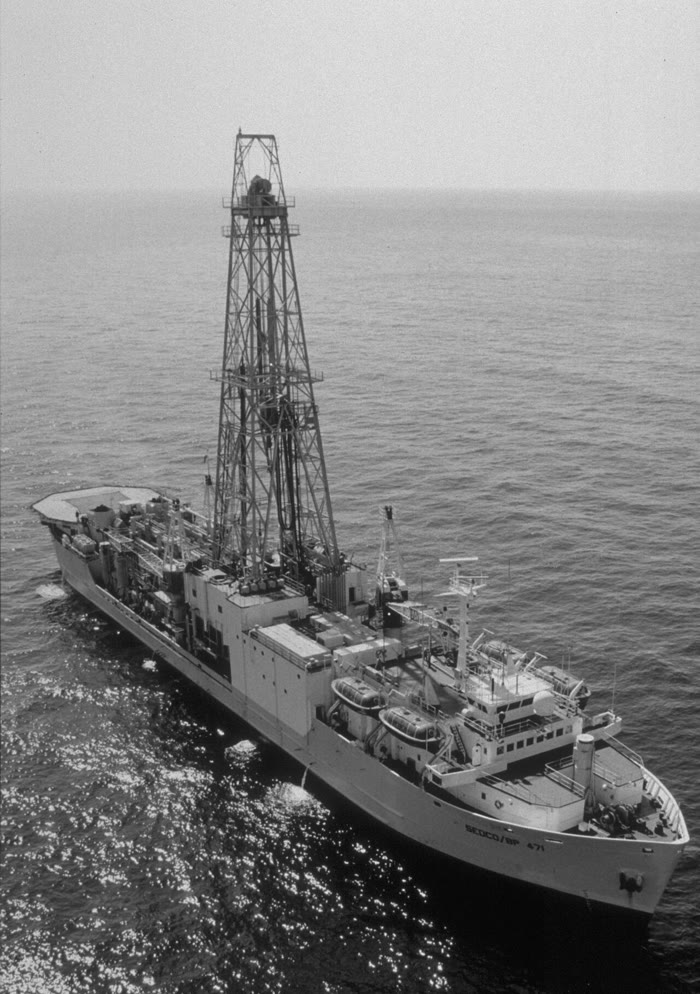
\includegraphics[width=0.36\linewidth]{images/book2/g11-odp-joides-resolution.jpg}

{\small Kapal bor \emph{JOIDES Resolution}, pengganti
\emph{Glomar Challenger}: menara yang tinggi itu adalah menara bornya, dan
kapal itu membawa lebih dari \qty{9000}{m} pipa bor.
Foto: Ocean Drilling Program, Texas A\&M University (domain publik).}
\end{omfigure}
% ledger: photo:g11-joides, usgs:glomar

Sejak itu, ribuan profil magnetik dan ratusan lubang bor telah disatukan
menjadi peta umur seluruh dasar samudra.

\begin{omfigure}
\begin{tikzpicture}
\begin{axis}[ommap, width=\linewidth, xtick=\empty, ytick=\empty, grid=none,
    axis background/.style={}, clip=true, name=map]
  \addplot graphics[xmin=-180, xmax=180, ymin=-90, ymax=90] {figdata/out/grade-11-seafloor_age.png};
  \addplot[black!60, line width=0.15pt] table {figdata/out/shared-geo-land.dat};
\end{axis}
\begin{axis}[at={(map.south)}, anchor=north, yshift=-0.35cm, scale only axis, width=0.55\linewidth, height=0.32cm,
    xmin=0, xmax=200, ymin=0, ymax=1, axis y line=none, axis x line*=bottom,
    xtick={0,20,...,180}, tick label style={font=\scriptsize},
    xlabel={umur dasar samudra (juta tahun); kelabu: bukan dasar samudra}, label style={font=\scriptsize},
    enlargelimits=false]
  \addplot graphics[xmin=0, xmax=200, ymin=0, ymax=1] {figdata/out/grade-11-seafloor_age-bar.png};
\end{axis}
\end{tikzpicture}

{\small Umur dasar samudra. Paling muda (merah) di sepanjang
punggung-punggung, dasar itu makin tua menjauhi punggung di kedua sisi; dasar
tertua (biru dan ungu) terletak di tepi-tepi samudra, berhadapan dengan
benua-benua dan di sepanjang palung-palung. Data: Seton dan kawan-kawan
(2020), dalam sel 1 derajat; garis daratan: Natural Earth.}
\end{omfigure}
% ledger: data:b2-seafloor-age, data:ne-land (map computed in figdata/grade-11/seafloor_age.py)

Peta itu menegaskan segalanya sekaligus. Di sepanjang setiap punggung
dasarnya muda, dan umurnya bertambah secara simetris menjauhi punggung itu.
Tidak ada dasar samudra yang lebih tua daripada sekitar \num{190} juta tahun:
yang tertua terletak di Pasifik barat dan di lepas pantai timur Amerika Utara
(beberapa cekungan kecil di Laut Tengah bagian timur dihitung terpisah). Umur
rata-rata dasar samudra sekitar \num{64} juta tahun, dan sekitar tiga
perempatnya lebih muda daripada 100 juta tahun --- sementara benua-benua
menyimpan batuan yang jauh lebih tua. Dasar samudra itu muda karena selalu
dibuat di punggung-punggung dan, seperti yang dilihat Hess, dihancurkan di
tempat lain: di mana, itulah pokok bahasan \cref{ch:g11:subduction-zones}.
% ledger: data:b2-seafloor-age (oldest_open_myr 192.5, share_younger_100 0.76 in figdata/grade-11/seafloor_age.py), seton:mean-age, usgs:hess

\section{Latihan}

\begin{exercise}[$\star$]\label{exo:g11:drift-to-spreading:1}
Definisikan \omterm{def:g11:drift-to-spreading:spreading}{pemekaran dasar samudra}. Apa perbedaan antara \omterm{def:g11:drift-to-spreading:spreading-rate}{laju pemekaran penuh}
dan laju setengah pemekaran sebuah punggung?
\end{exercise}

\begin{exercise}[$\star$]\label{exo:g11:drift-to-spreading:2}
Mengapa lava merekam arah medan Bumi hanya setelah mendingin di bawah sekitar
\qty{580}{\celsius}? Apa yang terjadi pada rekaman itu jika batuan itu kemudian
dipanaskan sampai \qty{700}{\celsius}?
\end{exercise}

\begin{exercise}[$\star$]\label{exo:g11:drift-to-spreading:3}
Sebuah perum gema mendengar gema pulsanya \qty{5.2}{s} setelah mengirimnya.
Dengan laju bunyi di air laut \qty{1500}{m/s}, berapa dalam dasar laut itu?
\end{exercise}

\begin{exercise}[$\star$]\label{exo:g11:drift-to-spreading:4}
Pada skala waktu polaritas dalam bab ini: berapa lama selang normal masa kini
telah berlangsung? Berapa lama peristiwa Jaramillo berlangsung? Berapa
pembalikan yang terjadi dalam lima juta tahun terakhir?
\end{exercise}

\begin{exercise}[$\star$]\label{exo:g11:drift-to-spreading:5}
Punggung-punggung tengah samudra panjangnya sekitar \qty{65000}{km}. Keliling
Bumi sekitar \qty{40000}{km}. Berapa kali punggung-punggung itu akan
mengelilingi Bumi?
\end{exercise}

\begin{exercise}[$\star\star$]\label{exo:g11:drift-to-spreading:6}
Pada sebuah profil magnetik, batas antara selang Brunhes dan Matuyama
(\num{0.78} juta tahun) terletak \qty{20}{km} dari sumbu punggung. Hitung laju
setengah dan laju penuhnya dalam sentimeter setahun.
\end{exercise}

\begin{exercise}[$\star\star$]\label{exo:g11:drift-to-spreading:7}
Pada profil lain, batas Gauss--Gilbert (\num{3.58} juta tahun) terletak
\qty{45}{km} di barat dan \qty{44}{km} di timur sumbu. Hitung laju setengah di
setiap sisi dan laju penuhnya. Apakah pemekarannya simetris?
\end{exercise}

\begin{exercise}[$\star\star$]\label{exo:g11:drift-to-spreading:8}
Lokasi 19 pengeboran tahun 1968 terletak \qty{990}{km} dari sumbu Punggung
Tengah Atlantik. Dengan laju setengah \qty{1.9}{cm} setahun, ramalkan umur
dasar di sana, lalu bandingkan dengan \num{49} juta tahun umur sedimen
tertuanya.
\end{exercise}

\begin{exercise}[$\star\star$]\label{exo:g11:drift-to-spreading:9}
Sebuah punggung memekar dengan laju setengah \qty{2}{cm} setahun. Dengan skala
waktu dalam bab ini, sebutkan jarak dari sumbu batas-batas pada 0.78, 0.99,
1.07, 1.77, dan 1.95 juta tahun, lalu gambarlah garis-garis di satu sisi,
dengan yang normal berwarna hitam.
\end{exercise}

\begin{exercise}[$\star\star$]\label{exo:g11:drift-to-spreading:10}
Umur rata-rata dasar samudra sekitar \num{64} juta tahun; umur Bumi sekitar
\num{4.6} miliar tahun. Berapa bagian dari umur Bumi itu? Argumen Hess yang
manakah yang didukungnya?
\end{exercise}

\begin{exercise}[$\star\star$]\label{exo:g11:drift-to-spreading:11}
Jelaskan, dengan sebuah gambar, mengapa pola garis-garis magnetik di satu sisi
punggung adalah bayangan cermin pola di sisi lainnya. Apa yang akan merusak
simetri ini?
\end{exercise}

\begin{exercise}[$\star\star\star$]\label{exo:g11:drift-to-spreading:12}
Misalkan punggung-punggung samudra, yang panjang seluruhnya \qty{65000}{km},
memekar dengan laju penuh rata-rata \qty{5}{cm} setahun.
\begin{enumerate}
  \item Berapa luas dasar samudra baru yang dibuatnya setiap tahun, dalam
        \unit{km^2}?
  \item Dasar samudra meliputi sekitar \qty{2.9e8}{km^2}. Berapa lama waktu
        yang diperlukan punggung-punggung itu untuk membuat seluas itu?
  \item Bandingkan dengan dasar samudra tertua, sekitar \num{190} juta tahun.
        Apa yang harus terjadi pada dasar samudra secepat dasar itu dibuat?
\end{enumerate}
\end{exercise}

\begin{exercise}[$\star\star\star$]\label{exo:g11:drift-to-spreading:13}
Peristiwa Jaramillo berlangsung dari \num{0.99} sampai \num{1.07} juta tahun
yang lalu. Berapa lebar garisnya di setiap sisi punggung yang laju setengahnya
\qty{1.25}{cm} setahun, dan di setiap sisi punggung yang laju setengahnya
\qty{7.5}{cm} setahun? Batuan yang termagnetisasi terletak sekitar \qty{3}{km}
di bawah permukaan laut. Jelaskan mengapa peristiwa itu tampak jelas pada
profil cepat dalam bab ini tetapi hampir tidak tampak pada profil lambat.
\end{exercise}

\begin{exercise}[$\star\star\star$]\label{exo:g11:drift-to-spreading:14}
Di lokasi-lokasi tahun 1968, sedimen setebal \qty{176}{m} di lokasi 16, yang
dasarnya berumur sekitar \num{11} juta tahun, dan hanya setebal \qty{72}{m} di
lokasi 20, yang berumur sekitar \num{67} juta tahun. Hitung laju rata-rata
penumpukan sedimen di setiap lokasi, dalam meter per sejuta tahun. Dapatkah
tebal sedimen dipakai untuk menentukan umur dasar samudra? Apa yang dipakai
sebagai gantinya?
\end{exercise}

\begin{exercise}[$\star\star\star$]\label{exo:g11:drift-to-spreading:15}
Pada sebuah profil yang melintasi punggung, batas \num{2.581} juta tahun
terletak \qty{58}{km} di barat dan \qty{70}{km} di timur sumbu.
\begin{enumerate}
  \item Hitung laju setengah di setiap sisi dan laju penuhnya.
  \item Dasar di timur sumbu dibuat lebih cepat daripada dasar di baratnya.
        Setelah 10 juta tahun dengan laju-laju ini, seberapa jauh dari sumbu
        dasar berumur itu akan terletak di setiap sisi?
  \item Jelaskan mengapa jarak di antara kedua batas itu memberikan laju penuh
        meskipun pemekarannya tidak simetris.
\end{enumerate}
\end{exercise}

\section{Soal: Umur Atlantik Selatan}

\begin{problem}[{Soal akhir pekan --- menentukan umur sebuah samudra dengan tiga cara}]
\label{pb:g11:drift-to-spreading:1}
% ledger: dsdp3:table5, dsdp3:rate, data:b2-seafloor-age, earth:Rmean, ics:base.Cretaceous
% (values computed in figdata/grade-11/sediment_ages.py and seafloor_age.py)
Pada tahun 1968 \emph{Glomar Challenger} mengebor tujuh lubang melintasi
Punggung Tengah Atlantik di dekat lintang \ang{30} LS. Tabel ini memberikan,
untuk setiap lokasi, jaraknya dari sumbu punggung, umur sedimen tertua di atas
basalt (dari fosil-fosilnya), dan, bila garis di bawahnya dikenali, umur garis
magnetik itu, dalam juta tahun.

\begin{center}
\small
\begin{tabular}{|c|c|c|c|}
\hline
lokasi & jarak dari sumbu (\unit{km}) & umur sedimen tertua & umur garis magnetik \\ \hline
16 & 191 & 11 & 9 \\ \hline
15 & 380 & 24 & 21 \\ \hline
18 & 506 & 26 & --- \\ \hline
17 & 643 & 33 & --- \\ \hline
14 & 727 & 40 & 38.5 \\ \hline
19 & 990 & 49 & 53 \\ \hline
20 & 1270 & 67 & 71 \\ \hline
\end{tabular}

{\small Data: Deep Sea Drilling Project, Leg 3 (1970); umur magnetik adalah
nilai tengah rentang-rentang yang diberikan di sana.}
\end{center}

\begin{center}
\begin{tikzpicture}
\begin{axis}[omrecord, width=0.82\linewidth, height=5.0cm, xmin=-50, xmax=16, ymin=0, ymax=140,
  xlabel={bujur di sepanjang \ang{30} LS (derajat; negatif: barat)}, ylabel={umur (juta tahun)},
  tick label style={font=\small}, label style={font=\small}, clip=false]
\addplot[omDef, line width=0.8pt] table[x=lon, y=age] {figdata/out/grade-11-seafloor_age-profile.dat};
\draw[omRidge, densely dashed] (axis cs:-13.8,0) -- (axis cs:-13.8,140);
\node[font=\scriptsize, text=omRidge, anchor=south] at (axis cs:-13.8,140) {sumbu punggung};
\fill (axis cs:-47.4,125.1) circle (1.5pt);
\node[font=\scriptsize, anchor=south west, inner sep=2pt] at (axis cs:-47.6,126) {Amerika Selatan};
\node[font=\scriptsize, anchor=north west, align=left] at (axis cs:14.2,135) {Afrika};
\fill (axis cs:13.8,129.8) circle (1.5pt);
\end{axis}
\end{tikzpicture}

{\small Umur dasar samudra di sepanjang paralel \ang{30} LS, dari Amerika
Selatan sampai Afrika; garisnya berhenti di tempat dasar samudra berakhir
berhadapan dengan setiap benua. Data: Seton dan kawan-kawan (2020).}
\end{center}

\medskip
\noindent\textbf{Bagian I --- Lokasi-lokasi pengeboran.}
\begin{enumerate}
  \item Lokasi manakah yang paling dekat dengan punggung, dan manakah yang
        paling jauh? Bagaimana perbandingan umurnya?
  \item Mengapa umur sedimen tertua yang terletak di atas basalt mendekati
        umur basalt itu sendiri? Apakah sedimen itu sedikit lebih tua atau
        sedikit lebih muda?
  \item Untuk setiap lokasi, hitung perbandingan jaraknya dengan umur sedimen
        tertuanya, dalam kilometer per sejuta tahun.
  \item Berapa rata-rata ketujuh perbandingan ini? Ubahlah ke sentimeter
        setahun.
  \item Lokasi 17 dan 18 terletak di timur punggung, yang lain di baratnya.
        Apakah lokasi-lokasi timur mengikuti kecenderungan yang sama dengan
        lokasi-lokasi barat? Apa artinya bagi pemekaran itu?
\end{enumerate}

\medskip
\noindent\textbf{Bagian II --- Laju dari sedimen.}
\begin{enumerate}[resume]
  \item Jika dasar samudra memekar dengan laju setengah $u$ yang tetap,
        bagaimana umur $t$ dasar itu bergantung pada jaraknya $d$ dari sumbu?
  \item Garis yang melalui titik asal dan paling cocok dengan titik-titik itu
        memiliki kemiringan $u = \sum d\,t / \sum t^2$. Untuk ketujuh lokasi,
        $\sum d\,t = \num{208276}$ dan $\sum t^2 = \num{10952}$ (dalam
        kilometer dan juta tahun). Hitung $u$ dalam kilometer per sejuta
        tahun dan dalam sentimeter setahun.
  \item Berapa \omterm{def:g11:drift-to-spreading:spreading-rate}{laju pemekaran penuh} Atlantik Selatan pada lintang ini?
  \item Para ilmuwan ekspedisi itu menulis bahwa lajunya ``sedikit kurang
        dari \qty{2}{cm} setahun''. Apakah kamu setuju?
  \item Dengan laju ini, ramalkan umur dasar di lokasi 20, lalu bandingkan
        dengan sedimen tertuanya.
\end{enumerate}

\medskip
\noindent\textbf{Bagian III --- Laju dari garis-garis magnetik.}
\begin{enumerate}[resume]
  \item Dari lokasi 16 saja (\qty{191}{km}, garis berumur 9 juta tahun),
        hitung laju setengahnya.
  \item Dari lokasi 20 saja (\qty{1270}{km}, garis berumur 71 juta tahun),
        hitung laju setengahnya.
  \item Untuk kelima lokasi yang memiliki umur magnetik,
        $\sum d\,t = \num{180329}$ dan
        $\sum t^2 = \num{9854}$. Hitung laju setengah yang terbaik.
  \item Berapa persen perbedaan laju dari fosil dan dari garis-garis magnetik?
        Apakah kedua metode itu sesuai?
  \item Mengapa penting bahwa kedua umur itu diperoleh dengan metode yang sama
        sekali berbeda?
\end{enumerate}

\medskip
\noindent\textbf{Bagian IV --- Sampai ke tepi samudra.}
\begin{enumerate}[resume]
  \item Di sepanjang \ang{30} LS, sumbu punggung terletak pada bujur
        \ang{13.8} BB dan dasar samudra berakhir berhadapan dengan Afrika pada
        \ang{13.8} BT. Berapa derajat bujur yang memisahkan keduanya?
  \item Pada bola berjari-jari \qty{6371}{km}, satu derajat bujur
        berukuran $\qty{111.2}{km} \times \cos(\text{lintang})$. Hitung
        panjang satu derajat pada \ang{30} LS, dan jarak dari sumbu ke tepi
        dasar samudra di dekat Afrika.
  \item Jika dasar samudra selalu memekar dengan laju pada Bagian II, berapa
        lama yang lalu dasar di tepi itu terbentuk?
  \item Peta umur, yang menentukan umur dasar tua melalui garis-garis
        magnetiknya, memberikan \num{130} juta tahun di tepi itu. Laju setengah
        rata-rata berapa yang diisyaratkannya? Apakah pembukaan awal samudra
        itu sedikit lebih cepat atau sedikit lebih lambat daripada pembukaan
        selama 66 juta tahun terakhir?
  \item Simpulkan: berapa umur dasar samudra tertua di dekat Afrika pada
        \ang{30} LS? Periode Kapur bermula sekitar \num{143} juta tahun yang
        lalu: dalam periode apakah Atlantik Selatan mulai membuka di sana?
\end{enumerate}
\end{problem}
